%! Author = Ian's PC
%! Date = 9/11/2023

% Preamble
\documentclass[11pt]{article}

% Packages
\usepackage{amsmath}
\usepackage{romannum}
\usepackage{graphicx}

% Document
\begin{document}
    Assignment 1 of CS376. Ian Chen, ic8683\newline
    
    \textbf{Part \Romannum{1}.}\newline

    \textbf{1. What are the three applications of image filtering?}\newline
    Hybrid images, where depending on how far you are from the image, you see different images.
    This is because a low pass filter is applied to the image in order to smooth the image, and a high pass filter is applied to the image
    to sharpen the image. The difference between the two creates the Laplacian of Gaussian.\newline
    Edge detection, where smoothening then calculating the gradient of the image will give us the edges of the image. This is useful to detext
    features in an image. Additionally, seam carving, an extension of edge detection, allows for smart resizing of an image based on removing seams
with the fewest edges\newline
    Template matching, where objects or sub images can be detected in another image.\newline

    \textbf{2. What is the difference between the mean filtering and the median filtering?}\newline
    Median filtering is non-linear and preserves edges while mean filtering is a linear filter that smoothes out the image and its edges.
    Median filtering retains all existing pixel values and doesn’t create new values. Median also removes spikes and salt \& pepper noise better
    than mean filters since the noise is usually the extremes of the filters. Mean filters are more sensitive to extrema in image intensities, so
    instead of removing the noise, the neighboring pixels may be negatively affected. Mean filters are useful to smooth out images for further analysis
    and manipulation, like detecting edges with a lower threshold or removing noise in images.\newline

    \textbf{3. In class, we talked about image smoothing followed by computing image gradients.
    Is it identical to computing image gradients first and then perform image smoothing on the resulting image gradients?}\newline
    No, it’s different, since the smoothing affects the gradients by decreasing the average gradient throughout the image. Paths in seam carving will
    likely change if blurring is done before the seam calculation vs. blurring after. My empirical tests also show this hypothesis to be true, as
    when blurring was applied to images then calculating the seam, the smallest cumulative gradient seam took a different path.\newline
    
    \textbf{4. How to take the advantage of the separability of a filter for fast image filtering calculation?}\newline
    We can convolve the rows and columns of the image separately, each using its own matrix operation. This makes the image filtering more
    efficient. This makes the 2D filter equivalent to two 1D convolutions. which will calculate faster since for a MxM image and NxN filter, with
    inseparable filters, it'll take O(M$^2$ $\cdot$ N$^2$), but the two 1D filters will take O(2 $\cdot$ N $\cdot$ M$^2$)\newline

    \textbf{5. In non-maximum suppressing, we detect the maximum pixel along the image gradient direction. Provide examples where this approach is sub-optimal.
    You can draw illustrations or provide results on real examples. Please provide a short justification (2-3 sentences) on why this is the case.}\newline
    Non-maximum suppression is a technique commonly used in edge detection algorithms like canny edge detection to thin out the edges and keep only
    the local maxima in the gradient direction. While it works well in many cases, there are situations where this approach can be sub-optimal.
    Here are a few examples: Wide edges-since the suppression may cause the line's width to be reduced, such as a bird's eye view of a highway
    system; Curved edges-since the suppression may cause the line to be straightened or fragmented, such as a curved road; Low contrast edges
    -since the gradient of the edges may be below the threshold limit for the edge detection algorithm, such as a dark road on a dark night.\newline
    
    \textbf{Extra credit (5points). So far we have covered filtering and edge detection for images. Please mention how to extend the idea to videos.
    Please discuss how to de-noise in both the spatial and/or temporal domain, how to compute gradients in the spatial and/or temporal domain,
        and how to detect ”edges” in the spatial and/or temporal domain.}\newline
    In videos, we can use the same techniques as in images, but we can also use temporal information to help us. Median filtering can be used to
    video frames just like images, but we can also use temporal information to help us. For example, if a pixel is an outlier with compared in the
    current frame to surrounding frames, we can replace it with the median of the surrounding frames. This is because the outlier is likely due to
    camera shake or sensor inconsistencies. We can also use temporal information to help us calculate gradients. For example, temporal edge
    detection methods analyze changes in pixel values across frames. We can track feature points over time and infer motion-based edges. This is
    especially useful for object tracking in videos. Detecting edges in videos can be similar to images, but now we can use the previous and
    next frames of the video to detect motion-based edges or track objects using the temporal domain. Video processing builds upon concepts in image
    processing, but also adds the dimension of time, which is another piece of information helpful to process the video.\newline

    \textbf{Part \Romannum{2}.}\newline
    
    \textbf{Question 1:}\newline
    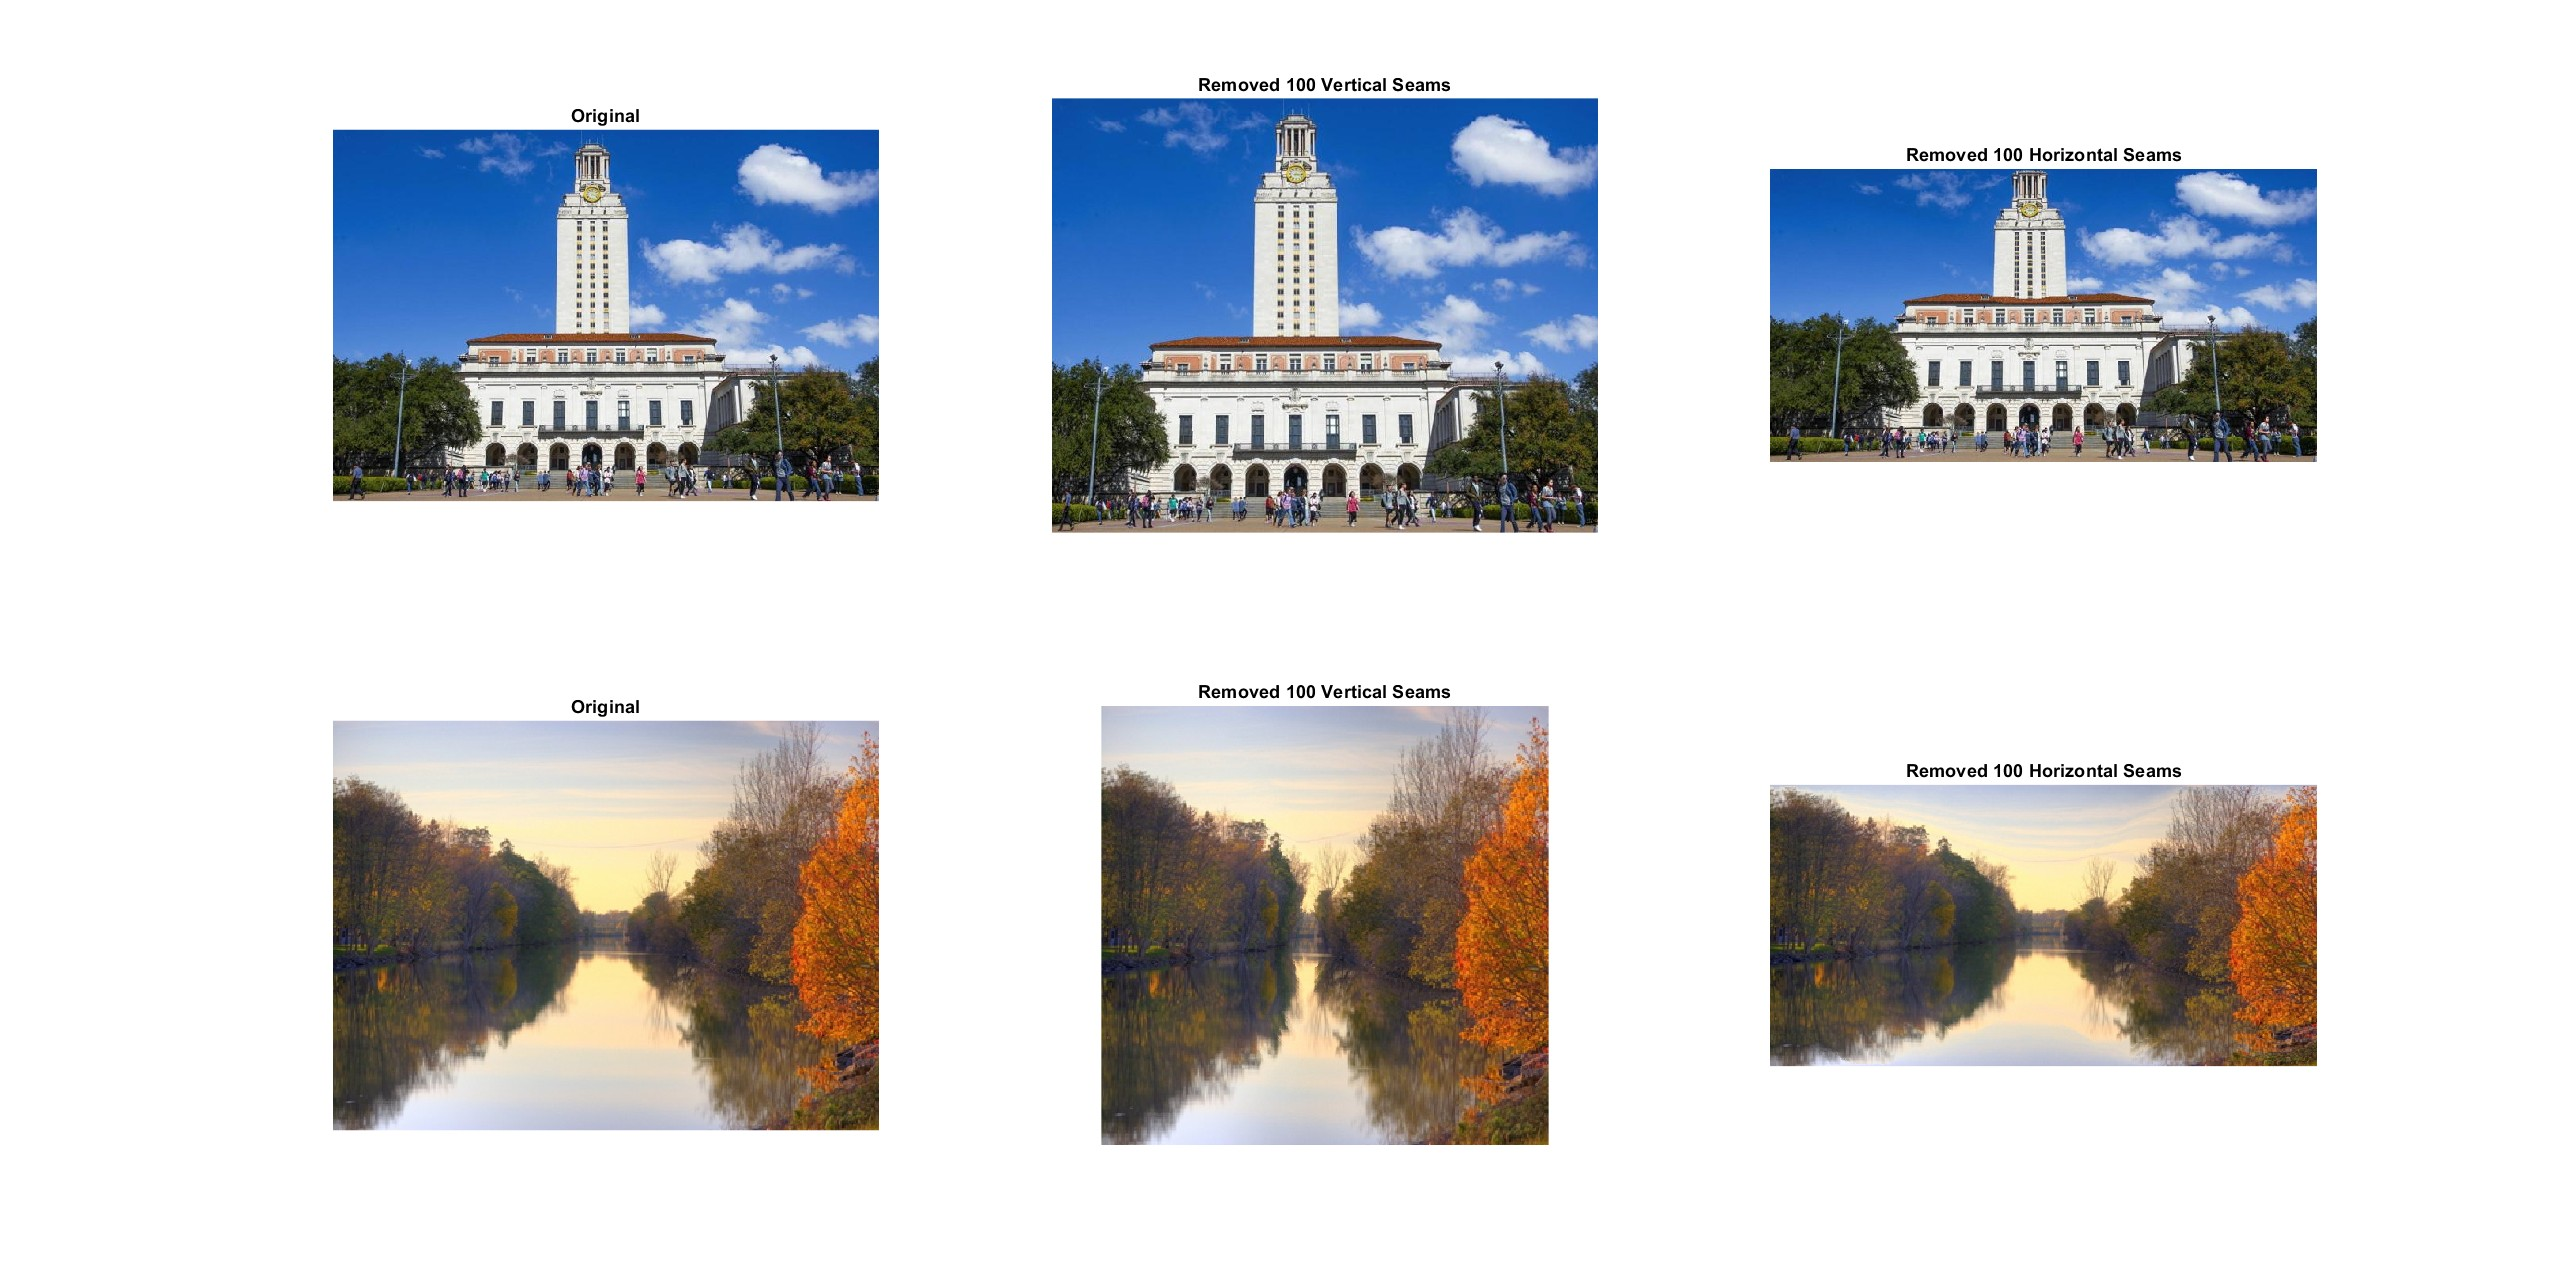
\includegraphics[width=\linewidth]{Part 2 Pictures/question1}\newline

    \textbf{Question 2:}\newline
    High-contrast regions or edges will have higher energy values, and areas with uniform color or texture will have lower energy values.
    The reason for these outputs is that on top of each object there's a
    triangle pointing to it, since for a object or background, the gradient
    is small, but, when edges to objects are detected through large
    gradients, the energy path will prioritize other paths which don't pass
    through many edges. Therefore, the seams will avoid the high-contrast regions and edges and pass through the uniform color or texture regions.\newline
    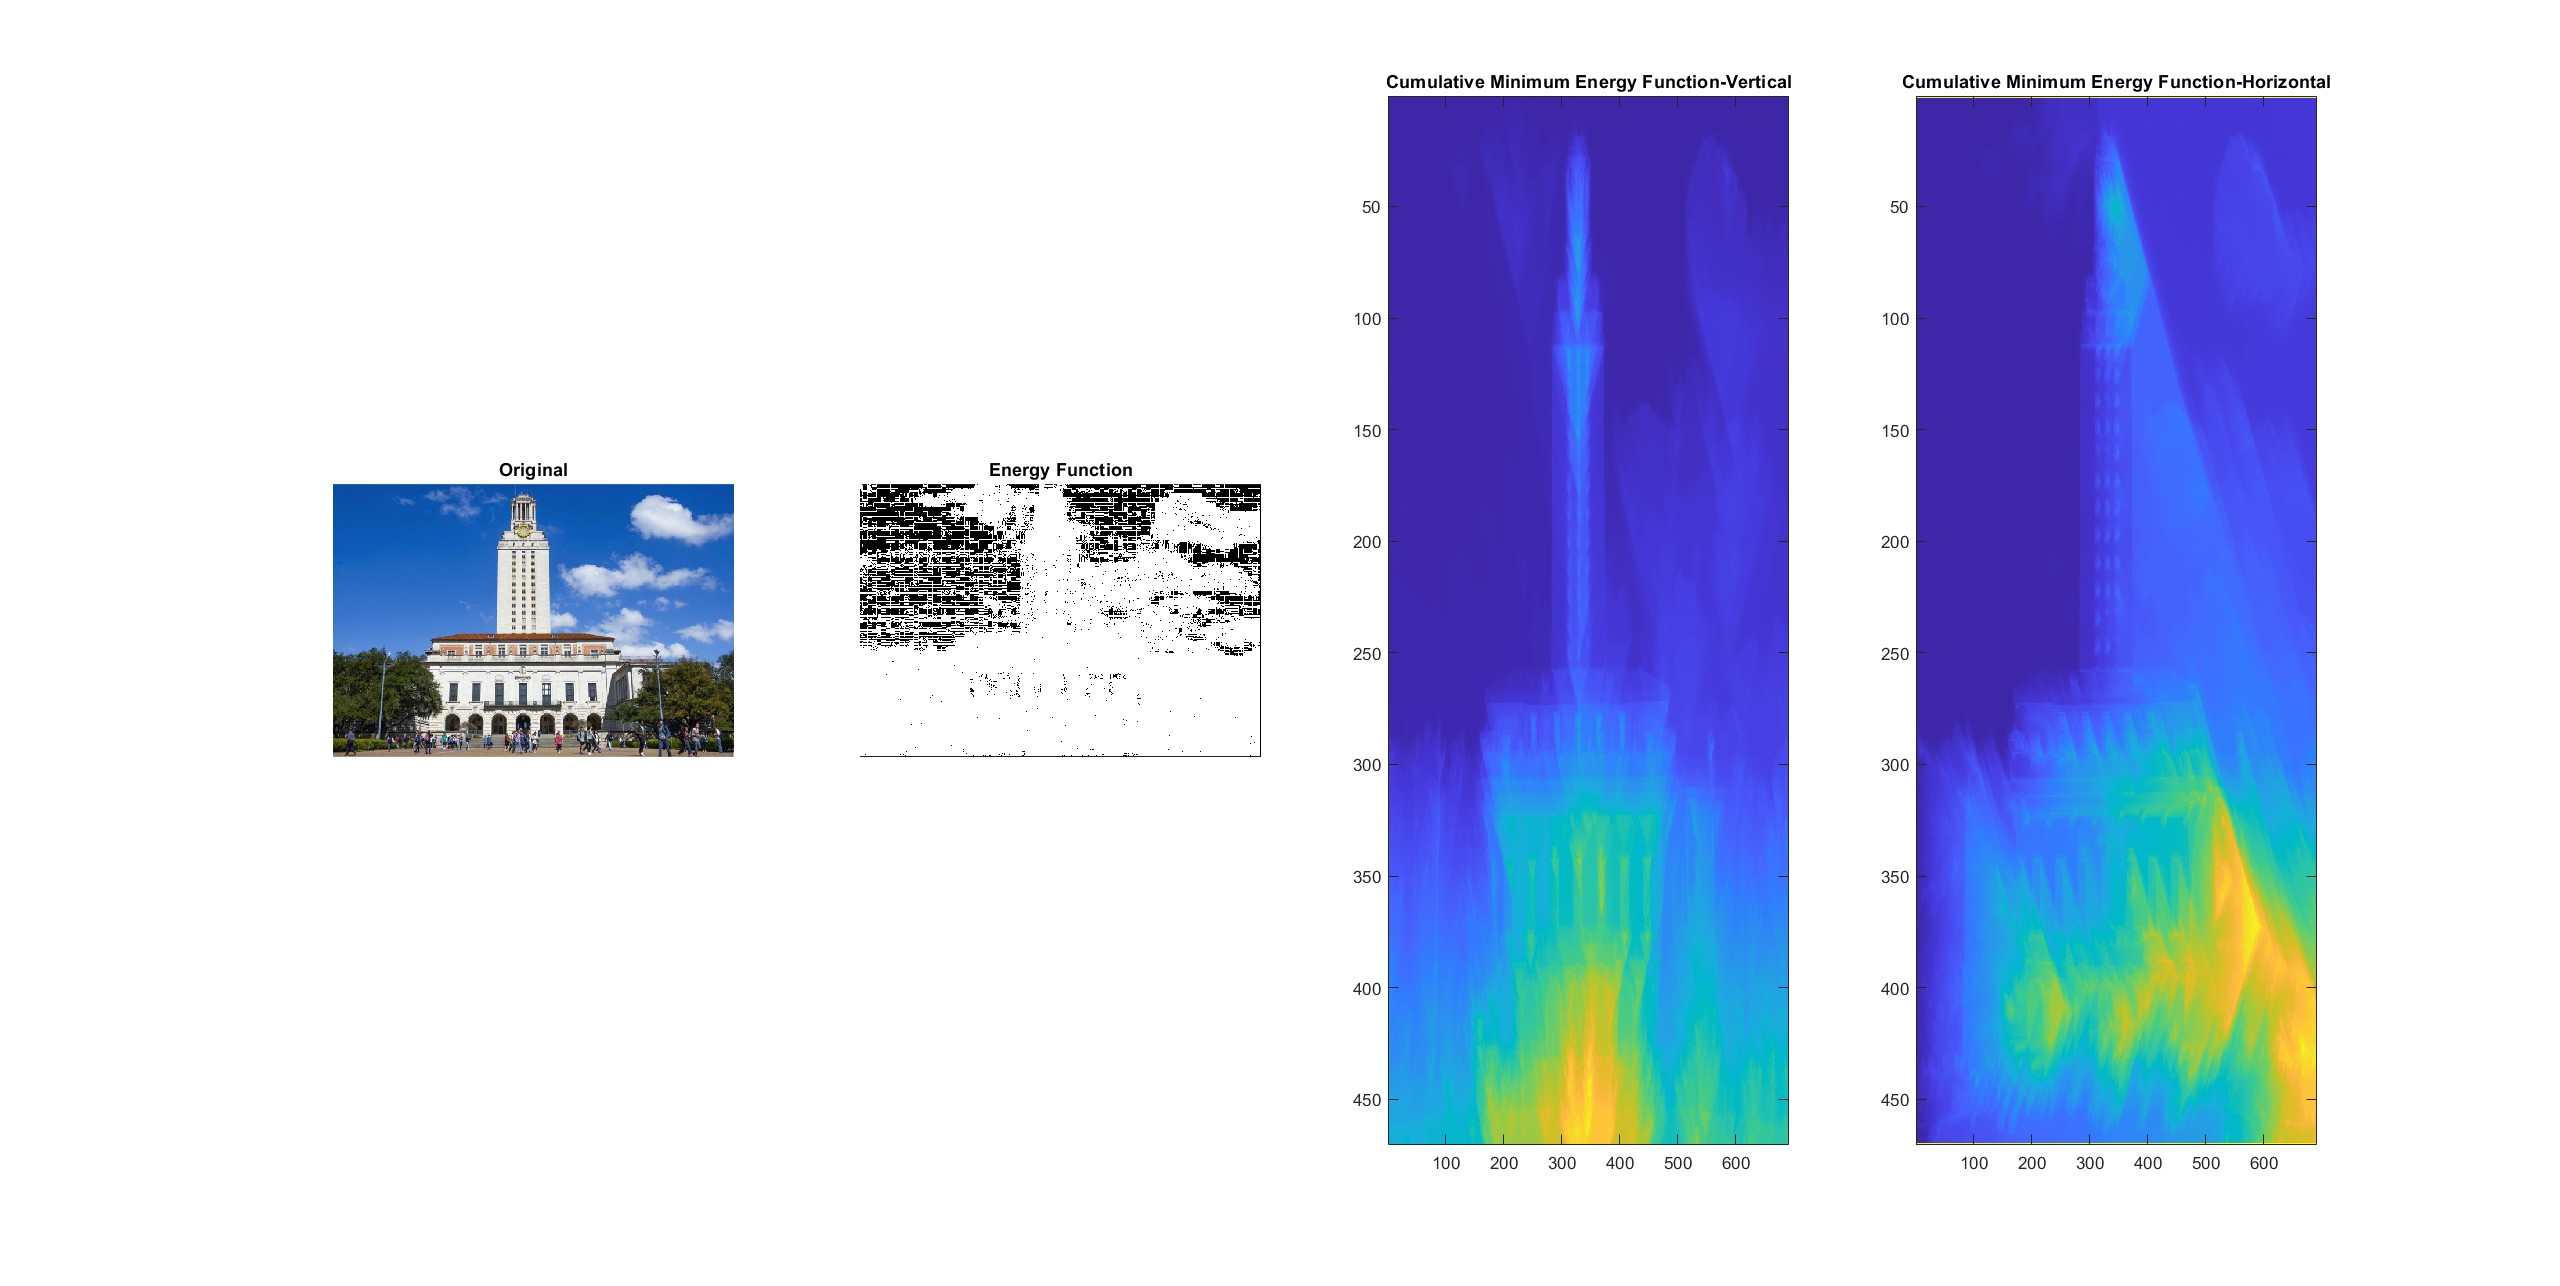
\includegraphics[width=\linewidth]{Part 2 Pictures/question2}\newline

    \textbf{Question 3:}\newline
    These are the optimal seams since they include the blue sky background,
    which is mostly the same color, therefore a small gradient. Therefore, their cumulative gradients will
    be small. However, in the vertical gradient, the trees in the foreground
    cover the entire bottom half, so the path passed through the patch which
    are mostly the same shade of the tree leaves. That's why the algorithm prioritizes passing through the blue sky and trees inctead of the UT
    tower and people, since those regions present many colors and objects. For the horizontal seam, since the blue sky extends throughout the
    entire length of the image, the seam will prioritize its path, since its mostly the same blue color.\newline
    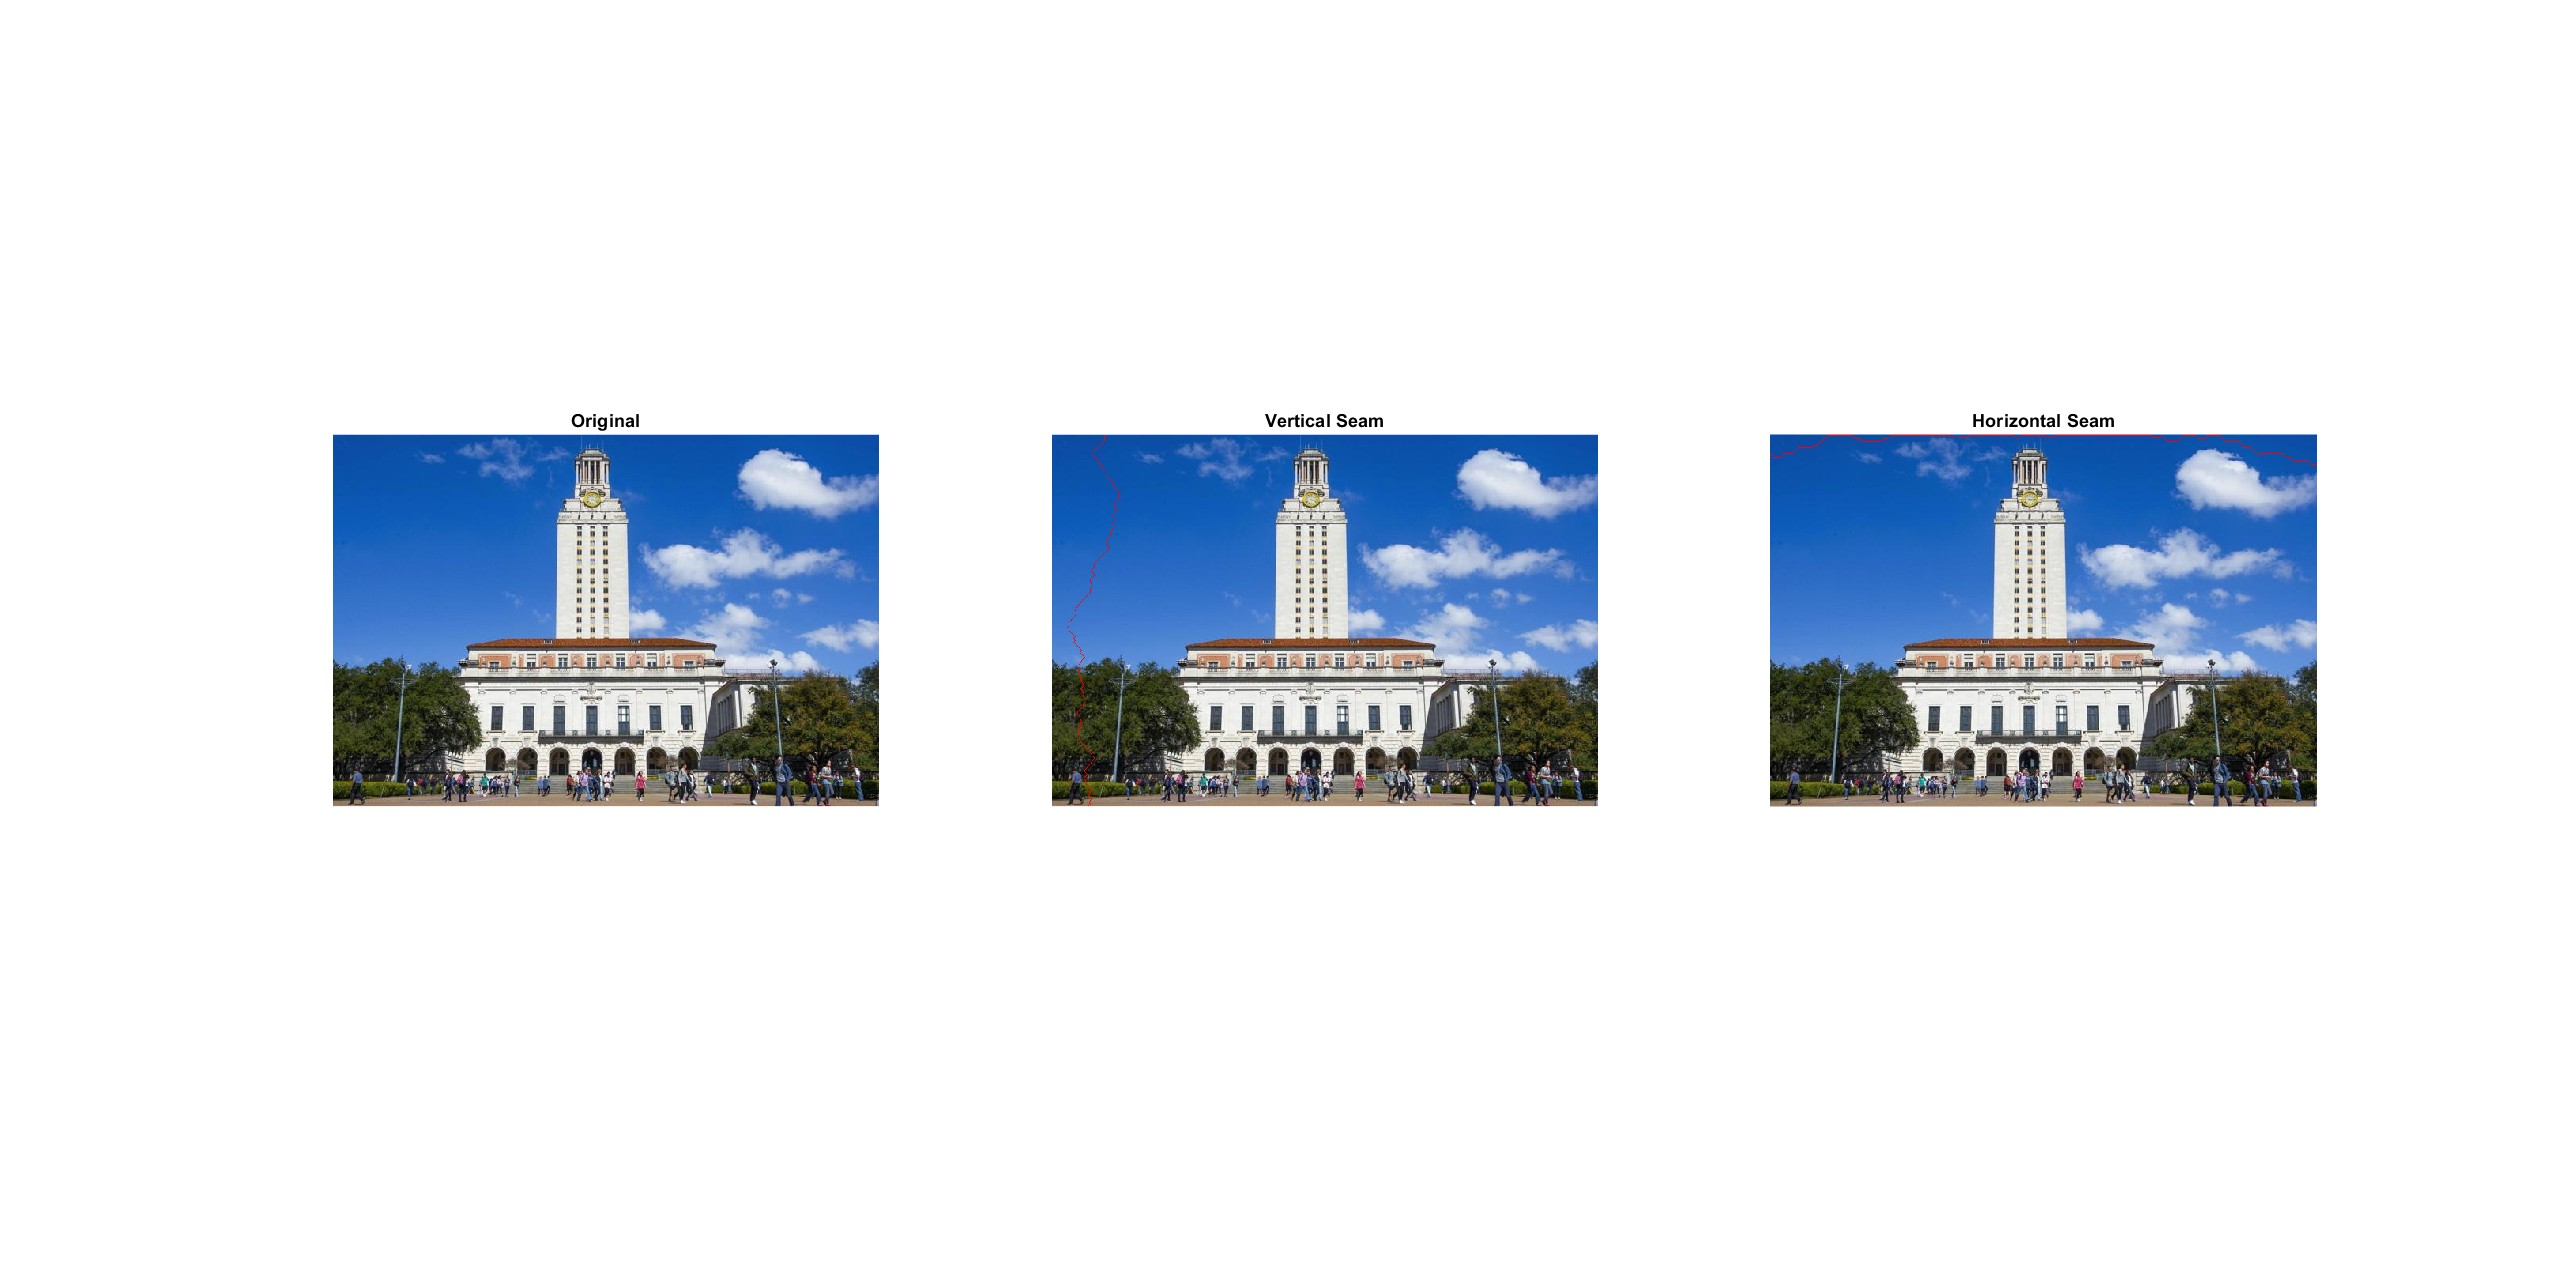
\includegraphics[width=\linewidth]{Part 2 Pictures/question3}\newline

    \textbf{Question 4:}\newline
    The results prove that blurring images first then calculating seams may
    produce different results then blurring images after calculating seams.
    This is because the gradients of each pixel now are smaller since its
    value is closer to its neighbors. Edges are suppressed, and areas or many pixel intensities where the algorithm previously avoided may have
    became a more uniform color and intensity.\newline
    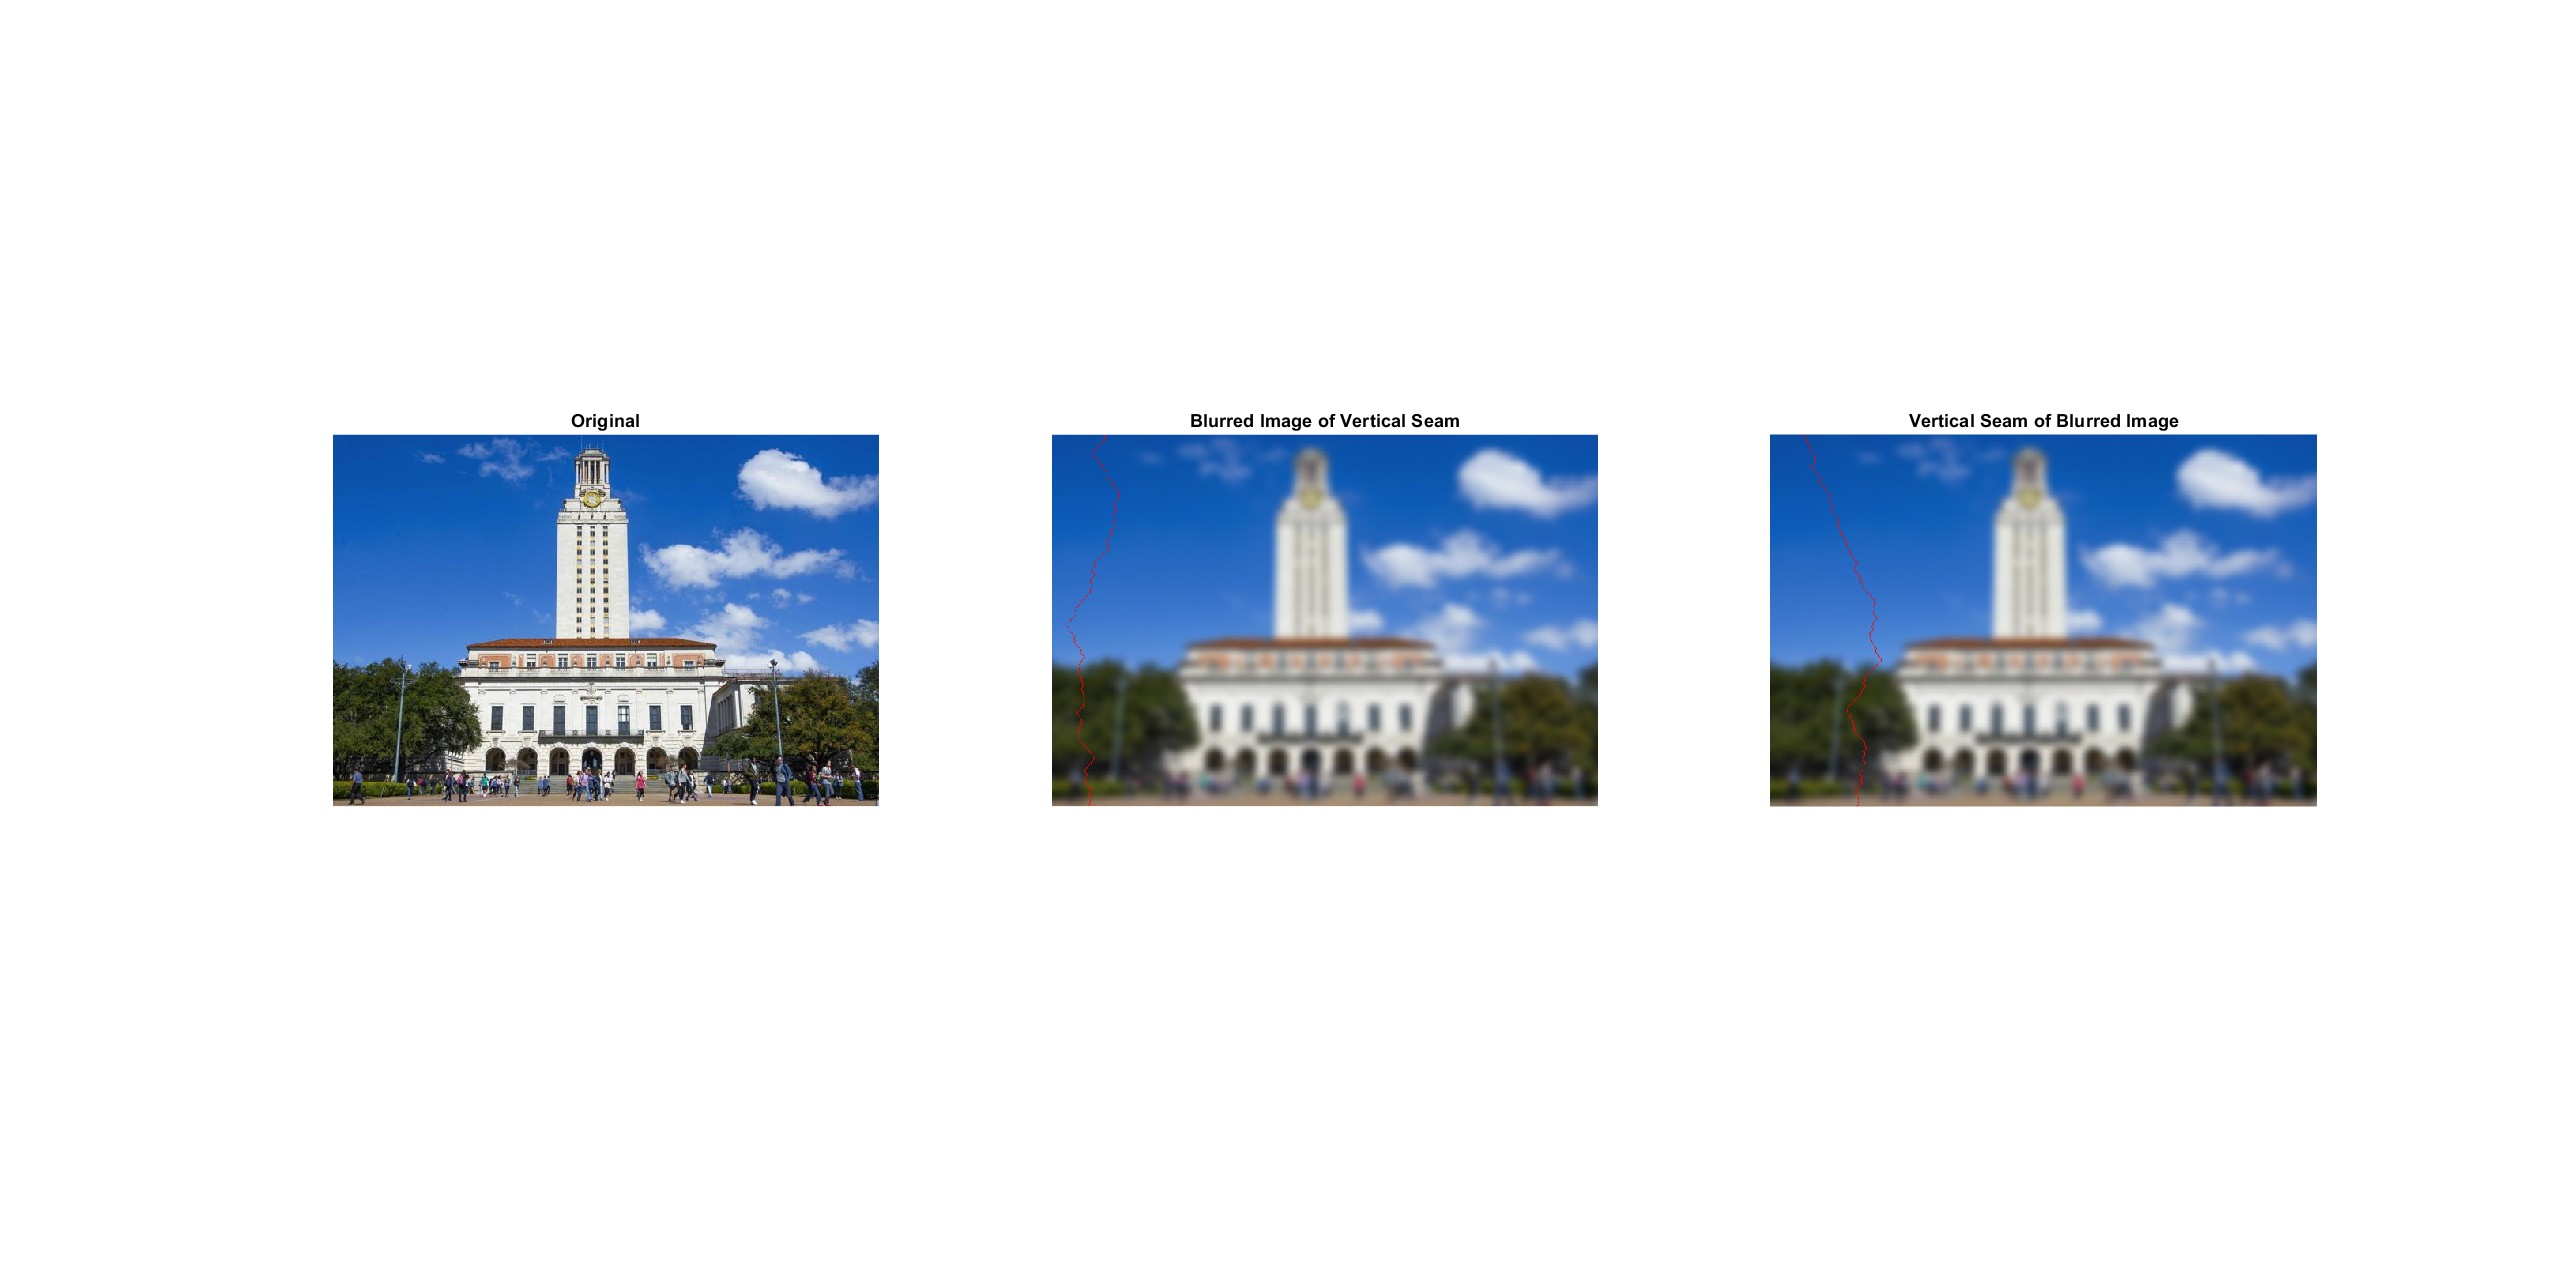
\includegraphics[width=\linewidth]{Part 2 Pictures/question4}\newline

    \textbf{Question 5:}\newline
    For the image of the Golden State Warriors winning the championship, I would argue that seam carving produced the worst results, since the
    faces were distorted, whereas the other two algorithms kept the faces structure the same. Seam carving stetched and ripped the faces, which is
    not ideal for this picture. For the image of the memory painting, I would argue that seam carving produced the best results, since it primarily
    enlarged objects while keeping their aspect ratio the same. Nearest neighbor resulted in a pixelated image, where edges were uneven and
    fragmented. Bicubic interpolation worked fine, where images kept their visual appearance, however the image was generally blurred and denoised
    , reducing the painting's authenticity. For the last image of the toucan, I would argue that all three algorithms performed well, since seam
    carving enlarged the foreground and the toucan, while preserving object structure and edge gradients. Nearest neighbor and bicubic
    interpolation shrank the image as expected, with nearest neighbor reducing edege quality and gradients a little worse than bicubix
    interpolation.\newline
    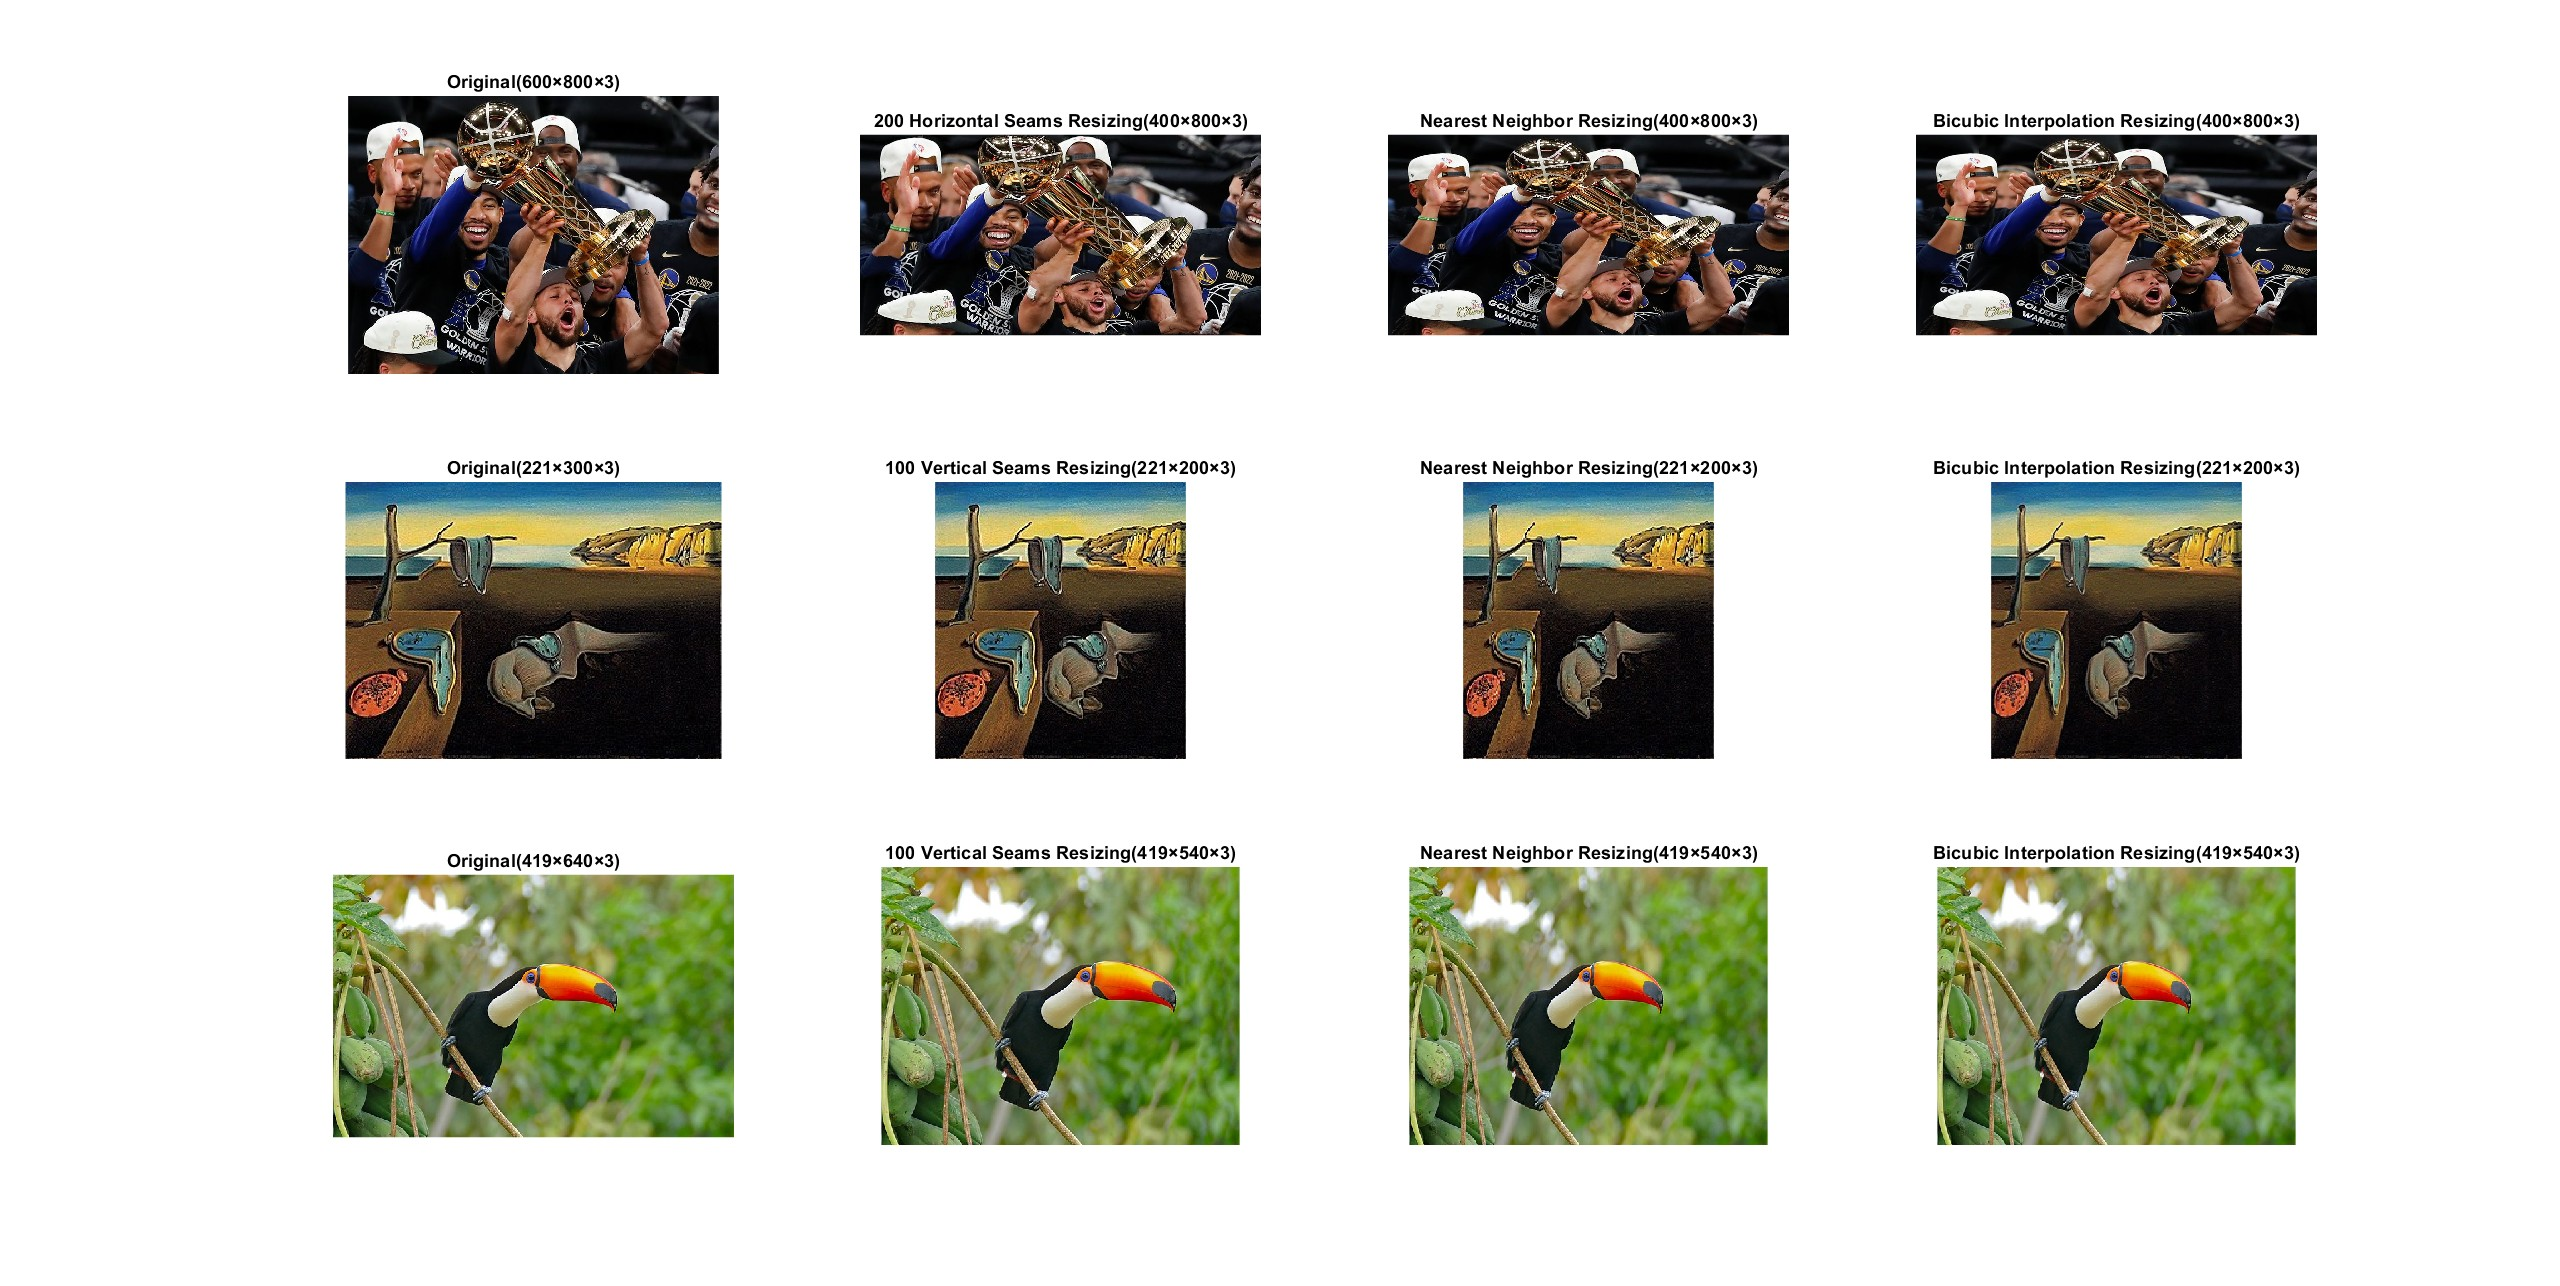
\includegraphics[width=\linewidth]{Part 2 Pictures/question5}\newline
\end{document}